%!TeX encoding = UTF-8
%!TeX program = xelatex
\documentclass[notheorems, aspectratio=149]{beamer}
% aspectratio: 1610, 149, 54, 43(default), 32

\usepackage{latexsym}
\usepackage{amsmath,amssymb}
\usepackage{mathtools}
\usepackage{color,xcolor}
\usepackage{graphicx}
\usepackage{algorithm}
\usepackage{amsthm}
\usepackage{lmodern} % 解决 font warning
% \usepackage[UTF8]{ctex}
\usepackage{animate} % insert gif

\usepackage{lipsum} % To generate test text 
\usepackage{ulem} % 下划线,波浪线

\usepackage{listings} % display code on slides; don't forget [fragile] option after \begin{frame}
	
	% ----------------------------------------------
	% tikx
	\usepackage{framed}
	\usepackage{tikz}
	\usepackage{pgf}
	\usetikzlibrary{calc,trees,positioning,arrows,chains,shapes.geometric,%
		decorations.pathreplacing,decorations.pathmorphing,shapes,%
		matrix,shapes.symbols}
	\pgfmathsetseed{1} % To have predictable results
	% Define a background layer, in which the parchment shape is drawn
	\pgfdeclarelayer{background}
	\pgfsetlayers{background,main}
	
	% define styles for the normal border and the torn border
	\tikzset{
		normal border/.style={orange!30!black!10, decorate, 
			decoration={random steps, segment length=2.5cm, amplitude=.7mm}},
		torn border/.style={orange!30!black!5, decorate, 
			decoration={random steps, segment length=.5cm, amplitude=1.7mm}}}
	
	% Macro to draw the shape behind the text, when it fits completly in the
	% page
	\def\parchmentframe#1{
		\tikz{
			\node[inner sep=2em] (A) {#1};  % Draw the text of the node
			\begin{pgfonlayer}{background}  % Draw the shape behind
				\fill[normal border] 
				(A.south east) -- (A.south west) -- 
				(A.north west) -- (A.north east) -- cycle;
	\end{pgfonlayer}}}
	
	% Macro to draw the shape, when the text will continue in next page
	\def\parchmentframetop#1{
		\tikz{
			\node[inner sep=2em] (A) {#1};    % Draw the text of the node
			\begin{pgfonlayer}{background}    
				\fill[normal border]              % Draw the ``complete shape'' behind
				(A.south east) -- (A.south west) -- 
				(A.north west) -- (A.north east) -- cycle;
				\fill[torn border]                % Add the torn lower border
				($(A.south east)-(0,.2)$) -- ($(A.south west)-(0,.2)$) -- 
				($(A.south west)+(0,.2)$) -- ($(A.south east)+(0,.2)$) -- cycle;
	\end{pgfonlayer}}}
	
	% Macro to draw the shape, when the text continues from previous page
	\def\parchmentframebottom#1{
		\tikz{
			\node[inner sep=2em] (A) {#1};   % Draw the text of the node
			\begin{pgfonlayer}{background}   
				\fill[normal border]             % Draw the ``complete shape'' behind
				(A.south east) -- (A.south west) -- 
				(A.north west) -- (A.north east) -- cycle;
				\fill[torn border]               % Add the torn upper border
				($(A.north east)-(0,.2)$) -- ($(A.north west)-(0,.2)$) -- 
				($(A.north west)+(0,.2)$) -- ($(A.north east)+(0,.2)$) -- cycle;
	\end{pgfonlayer}}}
	
	% Macro to draw the shape, when both the text continues from previous page
	% and it will continue in next page
	\def\parchmentframemiddle#1{
		\tikz{
			\node[inner sep=2em] (A) {#1};   % Draw the text of the node
			\begin{pgfonlayer}{background}   
				\fill[normal border]             % Draw the ``complete shape'' behind
				(A.south east) -- (A.south west) -- 
				(A.north west) -- (A.north east) -- cycle;
				\fill[torn border]               % Add the torn lower border
				($(A.south east)-(0,.2)$) -- ($(A.south west)-(0,.2)$) -- 
				($(A.south west)+(0,.2)$) -- ($(A.south east)+(0,.2)$) -- cycle;
				\fill[torn border]               % Add the torn upper border
				($(A.north east)-(0,.2)$) -- ($(A.north west)-(0,.2)$) -- 
				($(A.north west)+(0,.2)$) -- ($(A.north east)+(0,.2)$) -- cycle;
	\end{pgfonlayer}}}
	
	% Define the environment which puts the frame
	% In this case, the environment also accepts an argument with an optional
	% title (which defaults to ``Example'', which is typeset in a box overlaid
	% on the top border
	\newenvironment{parchment}[1][Example]{%
		\def\FrameCommand{\parchmentframe}%
		\def\FirstFrameCommand{\parchmentframetop}%
		\def\LastFrameCommand{\parchmentframebottom}%
		\def\MidFrameCommand{\parchmentframemiddle}%
		\vskip\baselineskip
		\MakeFramed {\FrameRestore}
		\noindent\tikz\node[inner sep=1ex, draw=black!20,fill=white, 
		anchor=west, overlay] at (0em, 2em) {\sffamily#1};\par}%
	{\endMakeFramed}
	
	% ----------------------------------------------
	
	\mode<presentation>{
		\usetheme{Warsaw}
		% Boadilla CambridgeUS
		% default Antibes Berlin Copenhagen
		% Madrid Montpelier Ilmenau Malmoe
		% Berkeley Singapore Warsaw
		%\usecolortheme{beaver}
		% beetle, beaver, orchid, whale, dolphin
		\useoutertheme{infolines}
		% infolines miniframes shadow sidebar smoothbars smoothtree split tree
		\useinnertheme{circles}
		% circles, rectanges, rounded, inmargin
	}
	% 设置 block 颜色
	\setbeamercolor{block title}{bg=red!30,fg=white}
	
	\newcommand{\reditem}[1]{\setbeamercolor{item}{fg=red}\item #1}
	
	% 缩放公式大小
	\newcommand*{\Scale}[2][4]{\scalebox{#1}{\ensuremath{#2}}}
	
	% 解决 font warning
	\renewcommand\textbullet{\ensuremath{\bullet}}
	
	% ---------------------------------------------------------------------
	% flow chart
	\tikzset{
		>=stealth',
		punktchain/.style={
			rectangle, 
			rounded corners, 
			% fill=black!10,
			draw=white, very thick,
			text width=6em,
			minimum height=2em, 
			text centered, 
			on chain
		},
		largepunktchain/.style={
			rectangle,
			rounded corners,
			draw=white, very thick,
			text width=10em,
			minimum height=2em,
			on chain
		},
		line/.style={draw, thick, <-},
		element/.style={
			tape,
			top color=white,
			bottom color=blue!50!black!60!,
			minimum width=6em,
			draw=blue!40!black!90, very thick,
			text width=6em, 
			minimum height=2em, 
			text centered, 
			on chain
		},
		every join/.style={->, thick,shorten >=1pt},
		decoration={brace},
		tuborg/.style={decorate},
		tubnode/.style={midway, right=2pt},
		font={\fontsize{10pt}{12}\selectfont},
	}
	% ---------------------------------------------------------------------
	
	% code setting
	\lstset{
		language=C++,
		basicstyle=\ttfamily\footnotesize,
		keywordstyle=\color{red},
		breaklines=true,
		xleftmargin=2em,
		numbers=left,
		numberstyle=\color[RGB]{222,155,81},
		frame=leftline,
		tabsize=4,
		breakatwhitespace=false,
		showspaces=false,               
		showstringspaces=false,
		showtabs=false,
		morekeywords={Str, Num, List},
	}
	
	% ---------------------------------------------------------------------
	
	%% preamble
	\title[LP in KG with MAGNA]{Link prediction in Knowledge Graph with Multi-Attention Graph Neural Networks}
	% \subtitle{The subtitle}
	\author[Nhut-Nam Le]{Presenter: Nhut-Nam Le$^{1}$}
	\institute[HCMUS]{$^{1}$Computer Science Department, Faculty of Information Technology, Univeristy of Science, VNU, HCM City, Vietnam}
	
	% -------------------------------------------------------------
	
	\begin{document}
		
		%% title frame
		\begin{frame}
			\titlepage
		\end{frame}
		\begin{frame}{Table of contents}
			\tableofcontents
		\end{frame}
		%% normal frame
		\section{Motivation}
		\begin{frame}{Multi-relational Graphs \& Self-Attention Mechanism}
			i) A knowledge graph is a directed labeled graph in which the labels have well-defined meanings. One important characteristic of KG is \textbf{incompleteness}
			
			ii) Self-Attention in GNNs let to \textbf{SOTA performance} on many Graph Representation Learning tasks 
			\begin{columns}
				\begin{column}{0.5\textwidth}
					\begin{figure}[H]
						\centering
						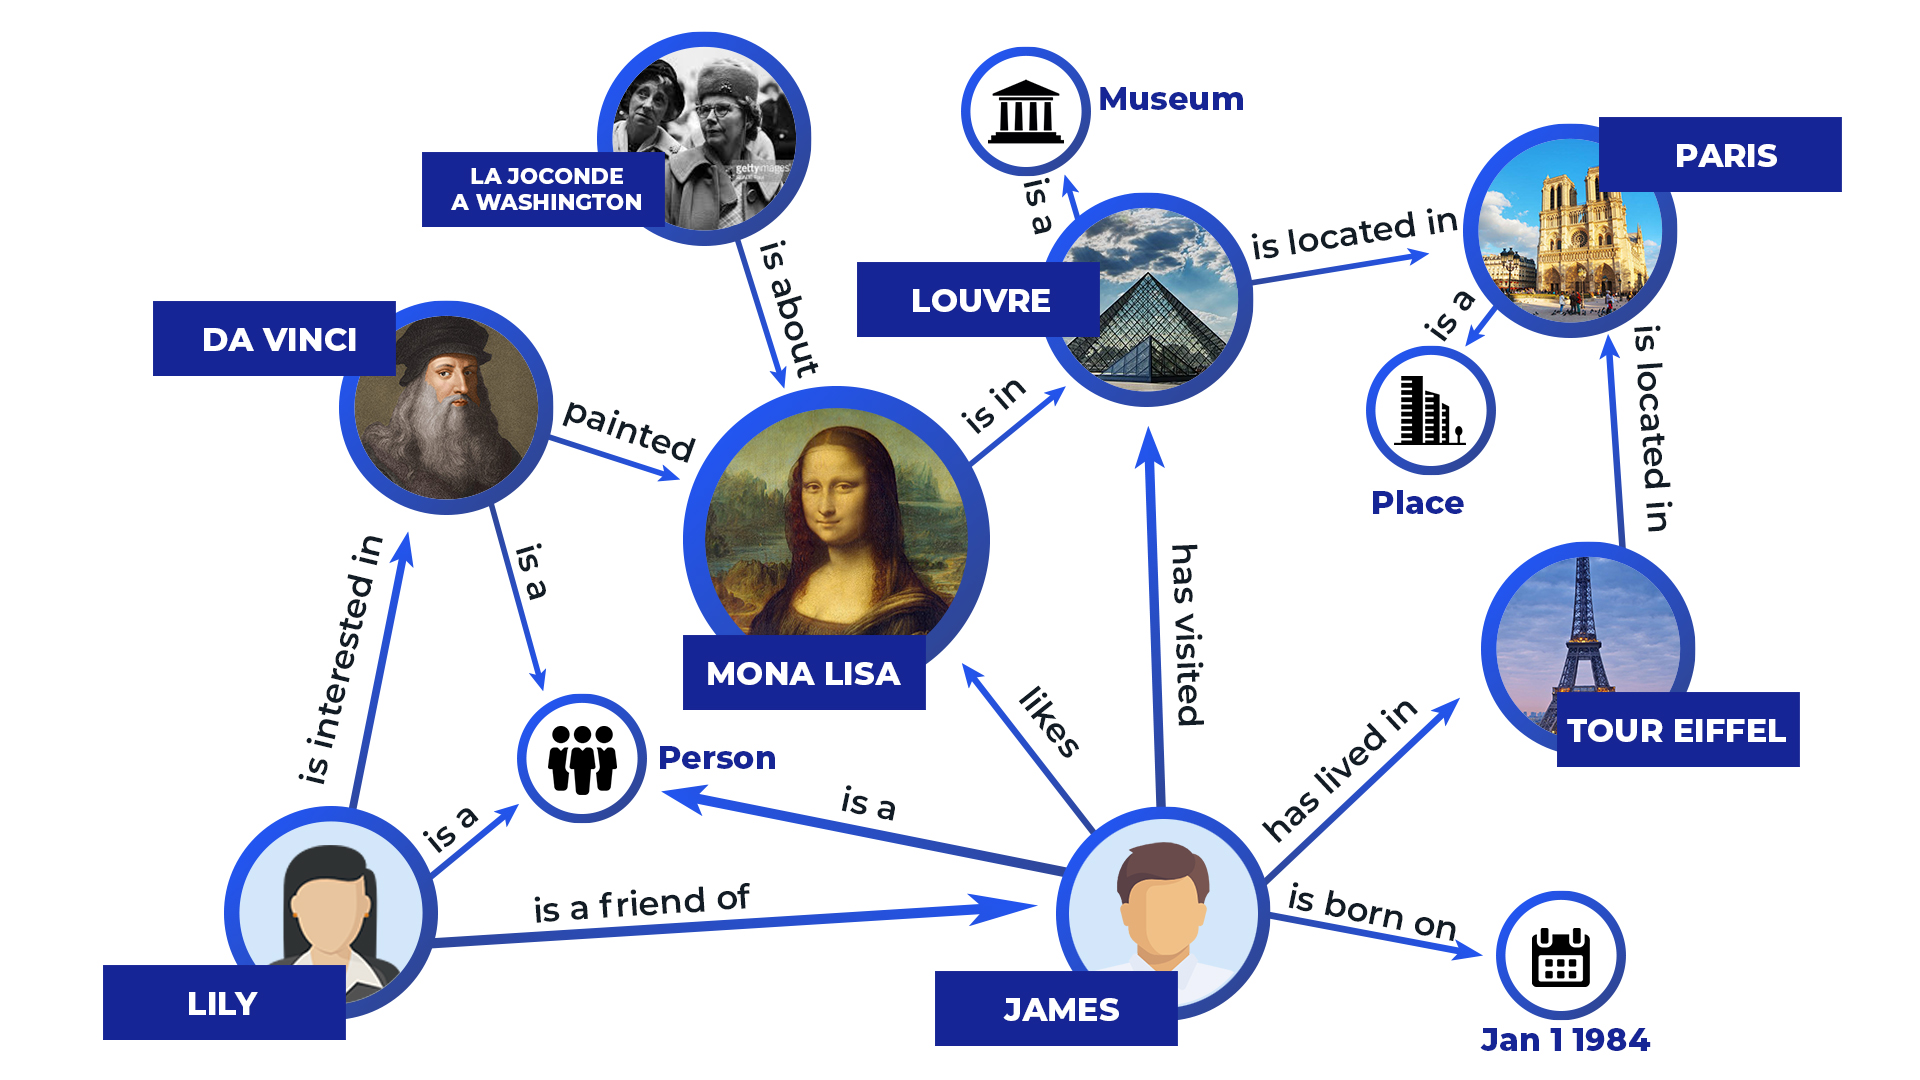
\includegraphics[width=1\linewidth]{figs/knowledge-graph.jpg}
						\caption{Visualize Knowledge Graph}
						\label{fig:writing-thesis}
					\end{figure}
				\end{column}
				\begin{column}{0.5\textwidth}  %%<--- here
					\begin{figure}[H]
						\centering
						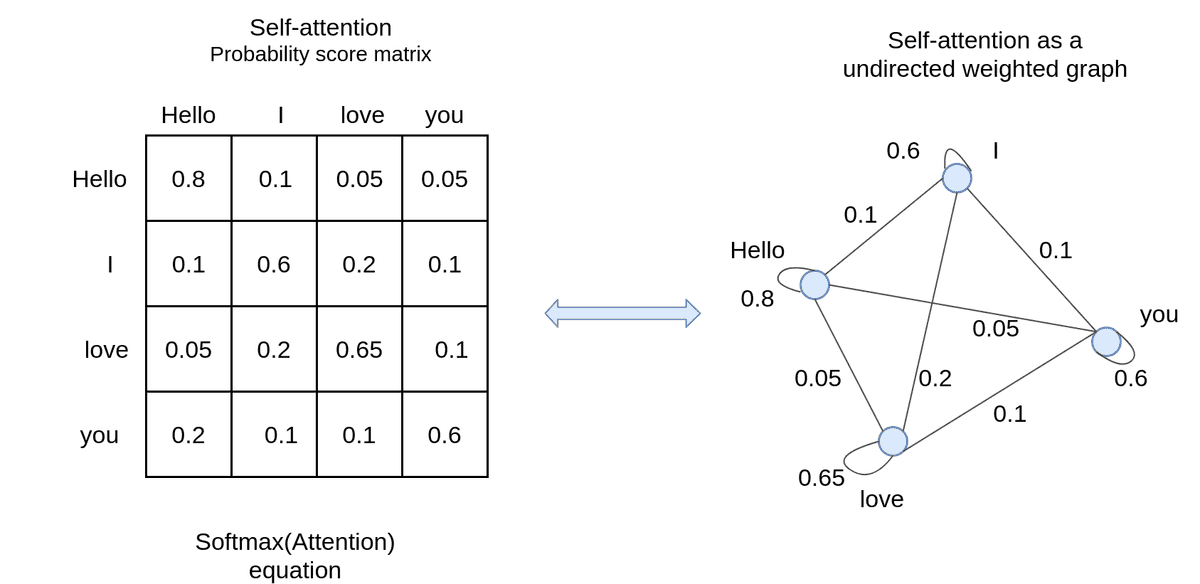
\includegraphics[width=1\linewidth]{figs/attention-graph.png}
						\caption{Self-attention}
						\label{fig:writing-thesis}
					\end{figure}
				\end{column}
			\end{columns}
		\end{frame}
		\begin{frame}{Attention mechanism limitation}
			\begin{columns}
				\begin{column}{0.5\textwidth}
					\begin{figure}[H]
						\centering
						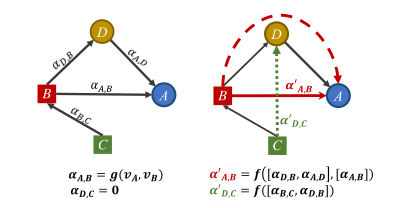
\includegraphics[width=1\linewidth]{figs/multihop-diffusion.png}
						\caption{Multi-hop attention diffusion}
						\label{fig:writing-thesis}
					\end{figure}
				\end{column}
				\begin{column}{0.5\textwidth}  %%<--- here
					\begin{itemize}
						\item Previous model using attention mechanism only consider nodes that directly connected by an edge. 
						\item The nodes in multi-hop neighbors of a node can provide important network context information
					\end{itemize}
				\end{column}
			\end{columns}
		\end{frame}
		\section{Preliminaries and problem statement}
		\begin{frame}{Preliminaries and problem statement}
			i) Knowledge graph (KG) is a heterogeneous graph. KG is
 defined by a set of entities (nodes) $v_i \in \mathcal{V}$, a set of relations (edges) $e = (v_i , r_k , v_j)$
			
			ii) KG completion refers to the task of predicting
 an entity that has a specific relation with another given entity [Bordes et al., 2013]
			\begin{itemize}
				\item Input: Given $(?, r, t)$ or $(h, r, ?)$ or $(h, ?, t)$
				\item Output: Give a list ranked contain entity/relation which can replace "?"
			\end{itemize}
		
			iii) A general Graph Neural Network (GNN) approach learns
an embedding that maps nodes and/or edge types into a continuous vector space.
		\end{frame}
		\section{Multi-hop Attention Graph Neural Network (MAGNA)}
		\subsection{Multi-hop Attention Diffusion}
		\begin{frame}{Multi-hop Attention Diffusion}
			\begin{itemize}
				\item Input: A set of triples $(v_i, r_k, v_j)$, where $v_i, v_j$ are nodes and $r_k$ is the edge type
			\end{itemize}
			i) Edge Attention Computation: Compute the attention scores on all edges
			
			Attention score $s$ for an edge $(v_i, r_k, v_j)$
			\begin{equation}
				s_{i, k, j}^{(l)} = \delta(\mathbf{v}_a^{(l)}\text{tanh}(\mathbf{W}_h^{(l)}\mathbf{h}_i^{(l)} || \mathbf{W}_t^{(l)}\mathbf{h}_j^{(l)} || \mathbf{W}_r^{(l)}\mathbf{r}_k^{(l)}))
			\end{equation}
		
			For each edge of the graph $\mathcal{G}$, applying Eq.1, obtain an attention score matrix $\mathbf{S}^{(l)}$
			\begin{equation}
				\mathbf{S}_{i, j}^{(l)} = \begin{cases}
					s_{i, j, k}^{(l)}, \text{ if } (v_i, r_k, v_j) \text{ appears in } \mathcal{G} \\
					- \infty, \text{ otherwise }
				\end{cases}
			\end{equation}
			Attention matrix
			\begin{equation}
				\mathbf{A}^{(l)} = \text{softmax}(\mathbf{S}^{(l)})
			\end{equation}
		\end{frame}
		\begin{frame}{Multi-hop Attention Diffusion}
			ii) Attention Diffusion for Multi-hop Neighbors: Enable attention between nodes that are not directly connected in the graph by using Attention diffusion procedure
			
			 Procedure processing based the powers of the 1-hop attention matrix $\mathbf{A}$
			 \begin{equation}
			 	\mathcal{A} = \sum_{i = 0}^{\infty} \theta_i \mathbf{A}^{i}
			 \end{equation}
		 Where $\sum_{i=0}^{\infty}\theta_i = 1$ and $\theta_i > 0$
		 
		 Implementation: Using geometric distribution $\theta_i = \alpha(1-\alpha)^{i}$, where $\alpha \in (0, 1]$
		 
		 If $\theta_0 = \alpha \in (0, 1]$, $\mathbf{A}^0 = \mathbf{I}$ => Personalized Page Rank (PPR)
		 
		 Graph attention
diffusion based feature aggregation:
		 \begin{equation}
		 	\text{AttDiff}(\mathcal{G}, \mathbf{H}^{(l)}, \Theta) = \mathcal{A}\mathbf{H}^{(l)}
		 \end{equation}
	 	Approximate $\mathcal{A}\mathbf{H}^{(l)}$ by defining a sequence which converges to the true value of $\mathcal{A}\mathbf{H}^{(l)}$ is $Z^{(K)}$ when $K \rightarrow \infty$: $Z^{(0)} = \mathbf{H}^{(l)}$,  $Z^{(k+1)} = (1-\alpha)\mathcal{A}Z^{(k)} + \alpha Z^{(0)}$
		\end{frame}
		\subsection{Multi-hop Attention based GNN Architecture}
		\begin{frame}{Multi-head Graph Attention Diffusion Layer}
			\begin{columns}
				\begin{column}{0.4\textwidth}
					\begin{figure}[H]
						\centering
						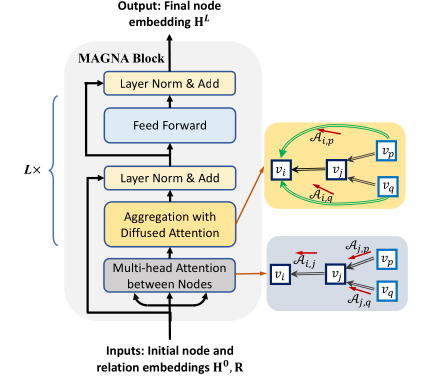
\includegraphics[width=1\linewidth]{figs/magna_architecture.png}
						\caption{MAGNA Architecture}
						\label{fig:writing-thesis}
					\end{figure}
				\end{column}
				\begin{column}{0.6\textwidth}  %%<--- here
					\textbf{Multi-head Graph Attention Diffusion Layer}
					\begin{gather*}
						\hat{\mathbf{H}}^{(l)} = \text{MultiHead}(\mathcal{G}, \widetilde{\mathbf{H}}^{(l)}) = \left(||_{i=1}^{M}\text{head}_i\right)\mathbf{W}_0 \\
						\text{head}_i = \text{AttDiff}(\mathcal{G}, \widetilde{\mathbf{H}}^{(l)}, \Theta), \widetilde{\mathbf{H}}^{(l)} = LN(\mathbf{H}^{(l)})
					\end{gather*}
					\textbf{Deep Aggregation}
					\begin{gather*}
						\hat{\mathbf{H}}^{(l+1)} = \hat{\mathbf{H}}^{(l)} + \mathbf{H}^{(l)}\\
						\mathbf{H}^{(l+1)} = \mathbf{W}_2^{(l)}\text{ReLU}(\mathbf{W}_1^{(l)}LN(\mathbf{H}^{(l+1)})) + \hat{\mathbf{H}}^{(l+1)}
					\end{gather*}
					MAGNA generalizes GAT:
					\begin{itemize}
						\item Removing the restriction of attending to direct neighbors
						\item Using layer normalization and deep aggregation to achieve
						higher expressive power
					\end{itemize}
				\end{column}
			\end{columns}
		\end{frame}
		\section{Experiments}
		\begin{frame}{Knowledge Graph Completion}
			\begin{figure}[H]
				\centering
				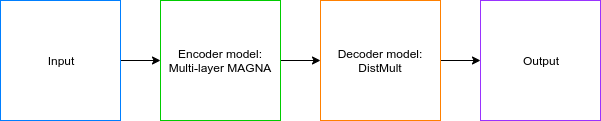
\includegraphics[width=1\linewidth]{figs/kgc.png}
				\caption{Encoder-Decoder framework for LP Problem}
				\label{fig:writing-thesis}
			\end{figure}
			\begin{itemize}
				\item The encoder applies the proposed MAGNA model to compute the entity embeddings
				\item The decoder makes link prediction given the embeddings
			\end{itemize}
		\end{frame}
		\section{Conclusion \& Improvement ideas}
		\begin{frame}{Conclusion \& Improvement ideas}
			\textbf{Conclusion} Multi-hop Attention Graph Neural Network, MAGNA, has two main advantages:
			\begin{itemize}
				\item Captures
long-range interactions between nodes that are not directly
connected but may be multiple hops away.
				\item The attention computation is context-dependent.
			\end{itemize}
			\textbf{Improvement ideas}
			\begin{itemize}
				\item Can we compose combine local features around a node with multi-hop attention using Graph Diffusion, then obtained entity embeddings and relation embeddings???
				\item Graph Diffusion is still complexity too much, can we improve this issue?
			\end{itemize}
		\end{frame}
		\begin{frame}{References}
			\nocite{*}
			\bibliography{references}\newpage\cleardoublepage
			\bibliographystyle{plain}
		\end{frame}
	\end{document}